% ============================================================
\chapter{R\'etropropagation et optimisation}
\label{ch:retropropagation}
% ============================================================

\begin{intuition}
La r\'etropropagation est l'algorithme qui permet au r\'eseau d'\emph{apprendre}. Elle r\'epond \`a une question simple : <<~Comment chaque poids influence-t-il l'erreur finale ?~>> En calculant efficacement tous les gradients par la r\`egle de cha\^ine, elle transforme un probl\`eme en apparence insoluble ($10^6$ param\`etres) en un calcul lin\'eaire en le nombre de param\`etres.
\end{intuition}

% ------------------------------------------------------------
\section{Descente de gradient}
\label{sec:gradient_descent}
\index{descente de gradient}

\subsection{Principe}

On cherche \`a minimiser la perte $\mathcal{L}(\theta)$ par rapport aux param\`etres $\theta$ :
\[
\theta^* = \argmin_\theta \mathcal{L}(\theta)
\]

La descente de gradient it\`ere la mise \`a jour :
\[
\theta_{t+1} = \theta_t - \eta \nabla_\theta \mathcal{L}(\theta_t)
\]
o\`u $\eta > 0$ est le \textbf{taux d'apprentissage}\index{taux d'apprentissage}.

\begin{center}
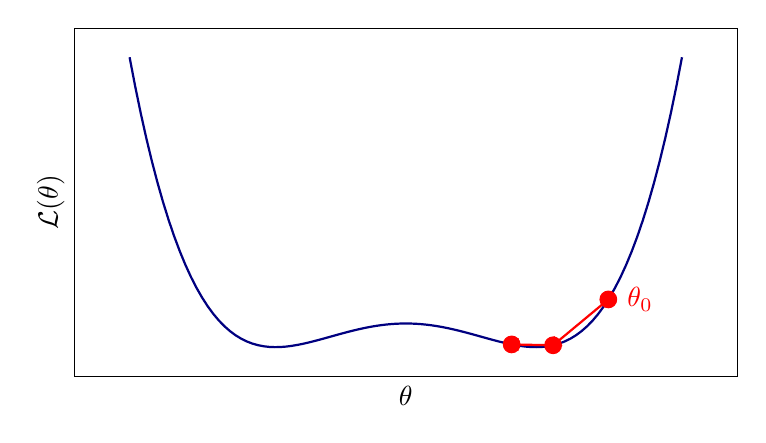
\begin{tikzpicture}
\begin{axis}[
    width=10cm, height=6cm,
    xlabel={$\theta$}, ylabel={$\mathcal{L}(\theta)$},
    domain=-3:3, samples=100,
    grid=major, grid style={gray!30},
    xtick=\empty, ytick=\empty
]
\addplot[NavyBlue, thick] {0.5*x^4 - 2*x^2 + 3};
% Flèches de descente
\addplot[only marks, mark=*, mark size=3pt, red] coordinates {(2.2, 0.5*2.2^4-2*2.2^2+3)};
\addplot[only marks, mark=*, mark size=3pt, red] coordinates {(1.6, 0.5*1.6^4-2*1.6^2+3)};
\addplot[only marks, mark=*, mark size=3pt, red] coordinates {(1.15, 0.5*1.15^4-2*1.15^2+3)};
\draw[->, red, thick] (axis cs:2.2, 0.5*2.2^4-2*2.2^2+3) -- (axis cs:1.6, 0.5*1.6^4-2*1.6^2+3);
\draw[->, red, thick] (axis cs:1.6, 0.5*1.6^4-2*1.6^2+3) -- (axis cs:1.15, 0.5*1.15^4-2*1.15^2+3);
\node[red, right] at (axis cs:2.3, 0.5*2.2^4-2*2.2^2+3) {$\theta_0$};
\end{axis}
\end{tikzpicture}
\end{center}

\subsection{Descente de gradient stochastique (SGD)}
\index{SGD}

En pratique, calculer $\nabla_\theta \mathcal{L}$ sur tout le dataset est co\^uteux. La SGD utilise des \textbf{mini-batchs}\index{mini-batch} $\mathcal{B} \subset \{1,\ldots,N\}$ de taille $B$ :
\[
\theta_{t+1} = \theta_t - \eta \cdot \frac{1}{|\mathcal{B}|} \sum_{i \in \mathcal{B}} \nabla_\theta \ell(f_\theta(\bm{x}_i), \bm{y}_i)
\]

\begin{proposition}
Le gradient stochastique est un estimateur non biais\'e du gradient complet :
\[
\E_{\mathcal{B}}\!\left[\frac{1}{|\mathcal{B}|}\sum_{i \in \mathcal{B}} \nabla_\theta \ell_i\right] = \nabla_\theta \mathcal{L}(\theta)
\]
Sa variance d\'ecro\^it en $\mathcal{O}(1/B)$.
\end{proposition}

% ------------------------------------------------------------
\section{R\'etropropagation}
\label{sec:backprop}
\index{r\'etropropagation}

\subsection{R\`egle de cha\^ine}
\index{r\`egle de cha\^ine}

Soit $f = f_L \circ f_{L-1} \circ \cdots \circ f_1$ une composition de fonctions. La r\`egle de cha\^ine donne :
\[
\frac{\partial \mathcal{L}}{\partial \theta^{(\ell)}} = \frac{\partial \mathcal{L}}{\partial \bm{h}^{(L)}} \cdot \frac{\partial \bm{h}^{(L)}}{\partial \bm{h}^{(L-1)}} \cdots \frac{\partial \bm{h}^{(\ell+1)}}{\partial \bm{h}^{(\ell)}} \cdot \frac{\partial \bm{h}^{(\ell)}}{\partial \theta^{(\ell)}}
\]

\begin{mathbox}[title=\textbf{D\'erivation de la r\'etropropagation pour un MLP}]
\textbf{Passe avant.} Pour $\ell = 1, \ldots, L$ :
\begin{align*}
\bm{z}^{(\ell)} &= W^{(\ell)} \bm{h}^{(\ell-1)} + \bm{b}^{(\ell)} \\
\bm{h}^{(\ell)} &= \sigma(\bm{z}^{(\ell)})
\end{align*}

\textbf{Passe arri\`ere.} On d\'efinit $\bm{\delta}^{(\ell)} = \frac{\partial \mathcal{L}}{\partial \bm{z}^{(\ell)}}$. Pour la derni\`ere couche :
\[
\bm{\delta}^{(L)} = \frac{\partial \mathcal{L}}{\partial \bm{h}^{(L)}} \odot \sigma'(\bm{z}^{(L)})
\]
Pour les couches $\ell = L-1, \ldots, 1$ (propagation arri\`ere) :
\[
\bm{\delta}^{(\ell)} = \left({W^{(\ell+1)}}^\top \bm{\delta}^{(\ell+1)}\right) \odot \sigma'(\bm{z}^{(\ell)})
\]
Les gradients des param\`etres sont alors :
\[
\frac{\partial \mathcal{L}}{\partial W^{(\ell)}} = \bm{\delta}^{(\ell)} {\bm{h}^{(\ell-1)}}^\top, \qquad \frac{\partial \mathcal{L}}{\partial \bm{b}^{(\ell)}} = \bm{\delta}^{(\ell)}
\]
\end{mathbox}

\subsection{Complexit\'e}

\begin{proposition}
La r\'etropropagation calcule \textbf{tous} les gradients en $\mathcal{O}(|\theta|)$, soit le m\^eme co\^ut que la passe avant. C'est un cas particulier de la \textbf{diff\'erentiation automatique en mode inverse}\index{diff\'erentiation automatique}.
\end{proposition}

\begin{center}
\begin{tikzpicture}[
    node distance=2cm,
    block/.style={rectangle, draw=NavyBlue, thick, rounded corners, minimum width=2cm, minimum height=0.8cm, fill=blue!10, align=center},
    >=Stealth
]
\node[block] (x) {$\bm{x}$};
\node[block, right=of x] (z1) {$\bm{z}^{(1)}$};
\node[block, right=of z1] (h1) {$\bm{h}^{(1)}$};
\node[block, right=of h1] (z2) {$\bm{z}^{(2)}$};
\node[block, right=of z2] (L) {$\mathcal{L}$};

\draw[->, thick, ForestGreen] (x) -- node[above, font=\small] {$W^{(1)}$} (z1);
\draw[->, thick, ForestGreen] (z1) -- node[above, font=\small] {$\sigma$} (h1);
\draw[->, thick, ForestGreen] (h1) -- node[above, font=\small] {$W^{(2)}$} (z2);
\draw[->, thick, ForestGreen] (z2) -- node[above, font=\small] {} (L);

\draw[<-, thick, BrickRed, bend right=30] (x.south) to node[below, font=\small] {$\bm{\delta}^{(0)}$} (z1.south);
\draw[<-, thick, BrickRed, bend right=30] (z1.south) to node[below, font=\small] {$\bm{\delta}^{(1)}$} (h1.south);
\draw[<-, thick, BrickRed, bend right=30] (h1.south) to node[below, font=\small] {} (z2.south);
\draw[<-, thick, BrickRed, bend right=30] (z2.south) to node[below, font=\small] {$\bm{\delta}^{(2)}$} (L.south);

\node[ForestGreen, above=0.3cm of h1] {\textbf{Passe avant} $\longrightarrow$};
\node[BrickRed, below=0.8cm of h1] {$\longleftarrow$ \textbf{Passe arri\`ere}};
\end{tikzpicture}
\end{center}

% ------------------------------------------------------------
\section{Graphe de calcul et autograd}
\label{sec:autograd}
\index{graphe de calcul}
\index{autograd}

PyTorch construit dynamiquement un \textbf{graphe de calcul} (DAG) lors de la passe avant. Chaque op\'eration enregistre comment calculer son gradient. L'appel \`a \py{loss.backward()} parcourt ce graphe en sens inverse.

\begin{codeblock}[title=\textbf{Autograd en action}]
\begin{minted}{python}
import torch

# Tenseurs avec suivi de gradient
x = torch.tensor([2.0, 3.0], requires_grad=True)
w = torch.tensor([1.0, -1.0], requires_grad=True)

# Passe avant : graphe construit automatiquement
z = x @ w          # produit scalaire
y = z.sigmoid()    # activation
loss = (y - 1)**2  # perte

# Passe arrière : tous les gradients calculés
loss.backward()
print(f"dL/dx = {x.grad}")   # gradient par rapport à x
print(f"dL/dw = {w.grad}")   # gradient par rapport à w
\end{minted}
\end{codeblock}

\begin{codeoutput}
\begin{verbatim}
dL/dx = tensor([-0.0689,  0.0689])
dL/dw = tensor([-0.1378,  0.2067])
\end{verbatim}
\end{codeoutput}

% ------------------------------------------------------------
\section{Optimiseurs avanc\'es}
\label{sec:optimiseurs}

\subsection{Momentum}
\index{momentum}

Le momentum accumule une moyenne mobile des gradients pass\'es pour acc\'el\'erer la convergence et lisser les oscillations :
\begin{align*}
\bm{v}_{t+1} &= \mu \bm{v}_t + \nabla_\theta \mathcal{L}(\theta_t) \\
\theta_{t+1} &= \theta_t - \eta \bm{v}_{t+1}
\end{align*}
avec $\mu \in [0,1)$ (typiquement $\mu = 0.9$).

\subsection{RMSProp}
\index{RMSProp}

RMSProp adapte le taux d'apprentissage par param\`etre en normalisant par la moyenne mobile des carr\'es des gradients :
\begin{align*}
\bm{s}_{t+1} &= \beta \bm{s}_t + (1-\beta)\,(\nabla_\theta \mathcal{L})^2 \\
\theta_{t+1} &= \theta_t - \frac{\eta}{\sqrt{\bm{s}_{t+1}} + \varepsilon} \odot \nabla_\theta \mathcal{L}
\end{align*}

\subsection{Adam}
\index{Adam}

Adam\cite{kingmaadam} combine le momentum et l'adaptation du taux d'apprentissage :

\begin{mathbox}[title=\textbf{Algorithme Adam}]
\begin{align*}
\bm{m}_{t+1} &= \beta_1 \bm{m}_t + (1-\beta_1)\,\bm{g}_t & \text{(premier moment)} \\
\bm{v}_{t+1} &= \beta_2 \bm{v}_t + (1-\beta_2)\,\bm{g}_t^2 & \text{(second moment)} \\
\hat{\bm{m}}_{t+1} &= \frac{\bm{m}_{t+1}}{1 - \beta_1^{t+1}} & \text{(correction du biais)} \\
\hat{\bm{v}}_{t+1} &= \frac{\bm{v}_{t+1}}{1 - \beta_2^{t+1}} & \\
\theta_{t+1} &= \theta_t - \frac{\eta}{\sqrt{\hat{\bm{v}}_{t+1}} + \varepsilon}\,\hat{\bm{m}}_{t+1}
\end{align*}
Valeurs par d\'efaut : $\beta_1 = 0.9$, $\beta_2 = 0.999$, $\varepsilon = 10^{-8}$.
\end{mathbox}

\subsection{AdamW}
\index{AdamW}

AdamW d\'ecouple la r\'egularisation $L_2$ de l'adaptation du taux d'apprentissage :
\[
\theta_{t+1} = (1 - \eta\lambda)\,\theta_t - \frac{\eta}{\sqrt{\hat{\bm{v}}_{t+1}} + \varepsilon}\,\hat{\bm{m}}_{t+1}
\]
C'est l'optimiseur standard pour l'entra\^inement des Transformers.

\subsection{Comparaison visuelle}

\begin{center}
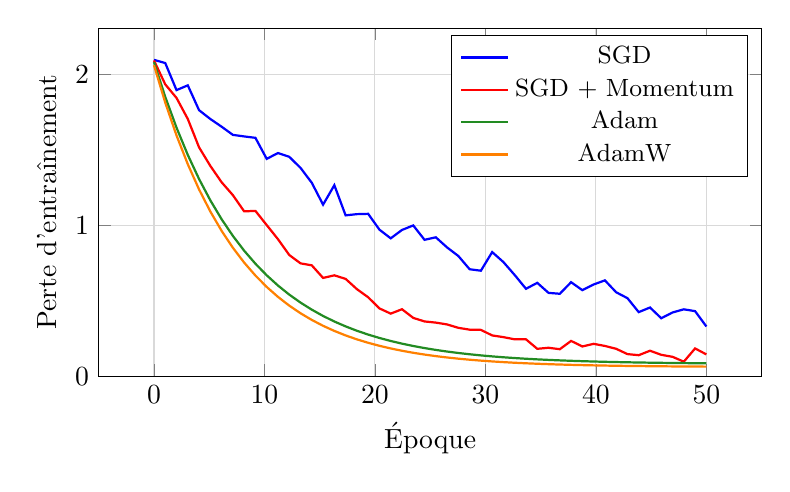
\begin{tikzpicture}
\begin{axis}[
    width=10cm, height=6cm,
    xlabel={\'Epoque}, ylabel={Perte d'entra\^inement},
    grid=major, grid style={gray!30},
    legend style={at={(0.98,0.98)}, anchor=north east, font=\small},
    ymin=0
]
% Courbes schématiques
\addplot[blue, thick, domain=0:50, samples=50] {2*exp(-0.04*x) + 0.15 + 0.1*rand};
\addlegendentry{SGD}
\addplot[red, thick, domain=0:50, samples=50] {2*exp(-0.08*x) + 0.1 + 0.05*rand};
\addlegendentry{SGD + Momentum}
\addplot[ForestGreen, thick, domain=0:50, samples=50] {2*exp(-0.12*x) + 0.08};
\addlegendentry{Adam}
\addplot[orange, thick, domain=0:50, samples=50] {2*exp(-0.13*x) + 0.06};
\addlegendentry{AdamW}
\end{axis}
\end{tikzpicture}
\end{center}

% ------------------------------------------------------------
\section{Planification du taux d'apprentissage}
\label{sec:lr_schedule}
\index{taux d'apprentissage!planification}

\subsection{D\'ecroissance par paliers (Step Decay)}

\[
\eta_t = \eta_0 \cdot \gamma^{\lfloor t / T \rfloor}
\]
avec $\gamma = 0.1$ tous les $T = 30$ \'epoques, par exemple.

\subsection{D\'ecroissance cosinus}
\index{cosine annealing}

\[
\eta_t = \eta_{\min} + \frac{1}{2}(\eta_{\max} - \eta_{\min})\left(1 + \cos\frac{\pi t}{T}\right)
\]

\subsection{Warmup lin\'eaire + d\'ecroissance cosinus}
\index{warmup}

Utilis\'e par d\'efaut pour les Transformers : augmentation lin\'eaire de $\eta$ pendant $T_w$ it\'erations, puis d\'ecroissance cosinus.

\begin{codeblock}[title=\textbf{Planificateurs en PyTorch}]
\begin{minted}{python}
from torch.optim.lr_scheduler import (
    StepLR, CosineAnnealingLR, OneCycleLR
)

optimizer = optim.AdamW(model.parameters(), lr=1e-3, weight_decay=0.01)

# Décroissance par paliers
scheduler_step = StepLR(optimizer, step_size=30, gamma=0.1)

# Cosine annealing
scheduler_cos = CosineAnnealingLR(optimizer, T_max=100, eta_min=1e-6)

# One-cycle (warmup + cosine decay)
scheduler_1cycle = OneCycleLR(
    optimizer, max_lr=1e-3, total_steps=len(train_loader) * EPOCHS
)

# Dans la boucle d'entraînement :
for epoch in range(EPOCHS):
    for X, y in train_loader:
        optimizer.zero_grad()
        loss = criterion(model(X.to(DEVICE)), y.to(DEVICE))
        loss.backward()
        optimizer.step()
        scheduler_1cycle.step()  # par itération pour OneCycle
    scheduler_cos.step()         # par époque pour CosineAnnealing
\end{minted}
\end{codeblock}

% ------------------------------------------------------------
\section{Probl\`emes de gradients}
\label{sec:gradient_problems}

\subsection{Gradient \'evanescent}
\index{gradient \'evanescent}

Dans un r\'eseau \`a $L$ couches avec des sigmo\"ides, le gradient de la couche $\ell$ contient le produit :
\[
\prod_{k=\ell+1}^{L} \sigma'(z^{(k)}) \cdot W^{(k)}
\]
Comme $|\sigma'(z)| \leq 1/4$, ce produit d\'ecro\^it exponentiellement avec $L - \ell$, emp\^echant l'apprentissage des premi\`eres couches.

\subsection{Gradient explosif}
\index{gradient explosif}

Si $\|W^{(k)}\| > 1/|\sigma'_{\max}|$, le produit cro\^it exponentiellement. Solution : le \textbf{gradient clipping}\index{gradient clipping} :
\[
\bm{g} \leftarrow \begin{cases}
\bm{g} & \text{si } \|\bm{g}\| \leq c \\
c \cdot \frac{\bm{g}}{\|\bm{g}\|} & \text{sinon}
\end{cases}
\]

\begin{codeblock}[title=\textbf{Gradient clipping en PyTorch}]
\begin{minted}{python}
# Après loss.backward(), avant optimizer.step()
torch.nn.utils.clip_grad_norm_(model.parameters(), max_norm=1.0)
\end{minted}
\end{codeblock}

\subsection{Solutions modernes}

\begin{enumerate}
\item \textbf{ReLU} : $\sigma'(z) = 1$ pour $z > 0$, pas d'att\'enuation.
\item \textbf{Connexions r\'esiduelles} (chapitre~\ref{ch:cnn}) : $\bm{h}^{(\ell)} = F(\bm{h}^{(\ell-1)}) + \bm{h}^{(\ell-1)}$.
\item \textbf{Normalisation} : BatchNorm, LayerNorm (chapitre~\ref{ch:regularisation}).
\item \textbf{Initialisation adapt\'ee} : Xavier, He (section~\ref{sec:init}).
\end{enumerate}

% ------------------------------------------------------------
\section{Impl\'ementation compl\`ete : r\'etropropagation manuelle}
\label{sec:backprop_manual}

\begin{codeblock}[title=\textbf{R\'etropropagation manuelle (sans autograd)}]
\begin{minted}{python}
import numpy as np

class ManualMLP:
    """MLP 2 couches avec backprop manuelle."""
    def __init__(self, d_in, d_hid, d_out):
        # Initialisation He
        self.W1 = np.random.randn(d_hid, d_in) * np.sqrt(2/d_in)
        self.b1 = np.zeros(d_hid)
        self.W2 = np.random.randn(d_out, d_hid) * np.sqrt(2/d_hid)
        self.b2 = np.zeros(d_out)

    def relu(self, z):
        return np.maximum(0, z)

    def softmax(self, z):
        e = np.exp(z - z.max(axis=1, keepdims=True))
        return e / e.sum(axis=1, keepdims=True)

    def forward(self, X):
        self.z1 = X @ self.W1.T + self.b1         # (N, d_hid)
        self.h1 = self.relu(self.z1)               # (N, d_hid)
        self.z2 = self.h1 @ self.W2.T + self.b2    # (N, d_out)
        self.probs = self.softmax(self.z2)          # (N, d_out)
        return self.probs

    def backward(self, X, y_onehot, lr=0.01):
        N = X.shape[0]
        # δ2 = ∂L/∂z2 = probs - y (pour CE + softmax)
        delta2 = (self.probs - y_onehot) / N        # (N, d_out)
        dW2 = delta2.T @ self.h1                     # (d_out, d_hid)
        db2 = delta2.sum(axis=0)                     # (d_out,)

        # δ1 = (δ2 @ W2) ⊙ ReLU'(z1)
        delta1 = (delta2 @ self.W2) * (self.z1 > 0)  # (N, d_hid)
        dW1 = delta1.T @ X                            # (d_hid, d_in)
        db1 = delta1.sum(axis=0)                       # (d_hid,)

        # Mise à jour
        self.W2 -= lr * dW2
        self.b2 -= lr * db2
        self.W1 -= lr * dW1
        self.b1 -= lr * db1

    def loss(self, y_onehot):
        return -np.mean(np.sum(y_onehot * np.log(self.probs + 1e-8),
                               axis=1))

# Test sur données synthétiques
np.random.seed(42)
X = np.random.randn(1000, 20)
y_true = (X[:, 0] + X[:, 1] > 0).astype(int)
y_oh = np.eye(2)[y_true]

mlp = ManualMLP(20, 64, 2)
for epoch in range(100):
    mlp.forward(X)
    if epoch % 20 == 0:
        acc = (mlp.probs.argmax(1) == y_true).mean()
        print(f"Epoch {epoch:3d} | Loss: {mlp.loss(y_oh):.4f}"
              f" | Acc: {acc:.4f}")
    mlp.backward(X, y_oh, lr=0.1)
\end{minted}
\end{codeblock}

\begin{codeoutput}
\begin{verbatim}
Epoch   0 | Loss: 0.7234 | Acc: 0.4930
Epoch  20 | Loss: 0.2156 | Acc: 0.9240
Epoch  40 | Loss: 0.1052 | Acc: 0.9670
Epoch  60 | Loss: 0.0614 | Acc: 0.9810
Epoch  80 | Loss: 0.0402 | Acc: 0.9880
\end{verbatim}
\end{codeoutput}

% ------------------------------------------------------------
\section{\'Etude d'ablation : optimiseurs}
\label{sec:ablation_optim}

\begin{codeblock}[title=\textbf{Comparaison d'optimiseurs sur MNIST}]
\begin{minted}{python}
optimizers = {
    "SGD":          optim.SGD(model.parameters(), lr=0.01),
    "SGD+Momentum": optim.SGD(model.parameters(), lr=0.01, momentum=0.9),
    "Adam":         optim.Adam(model.parameters(), lr=1e-3),
    "AdamW":        optim.AdamW(model.parameters(), lr=1e-3,
                                weight_decay=0.01),
}

for name, opt in optimizers.items():
    model_copy = MLP().to(DEVICE)
    opt = type(opt)(model_copy.parameters(), **opt.defaults)
    # Entraîner 10 époques, enregistrer loss et accuracy
    history = train_and_eval(model_copy, opt, train_loader,
                             test_loader, epochs=10)
    print(f"{name:15s} | Final Acc: {history['test_acc'][-1]:.4f}")
\end{minted}
\end{codeblock}

\begin{codeoutput}
\begin{verbatim}
SGD             | Final Acc: 0.9532
SGD+Momentum    | Final Acc: 0.9721
Adam            | Final Acc: 0.9793
AdamW           | Final Acc: 0.9801
\end{verbatim}
\end{codeoutput}

% ------------------------------------------------------------
\section{Connexion \`a l'\'etat de l'art}
\label{sec:sota_optim}

\begin{sota}
\begin{itemize}
\item \textbf{LAMB/LARS} (You et al., 2020) : optimiseurs adapt\'es pour l'entra\^inement distribu\'e avec de tr\`es grands batchs ($B > 8192$).
\item \textbf{Lion} (Chen et al., 2024) : optimiseur d\'ecouvert par recherche \'evolutionnaire, utilisant uniquement le signe du gradient, plus efficace en m\'emoire qu'Adam.
\item \textbf{Muon} (Jordan et al., 2024) : optimiseur bas\'e sur l'orthogonalisation du momentum, am\'eliorant la convergence pour les grands mod\`eles de langage.
\item \textbf{$\mu$P} (Yang \& Hu, 2022) : param\'etrisation maximale permettant de transf\'erer les hyperparamètres d'un petit mod\`ele vers un grand mod\`ele.
\end{itemize}
\end{sota}

% ------------------------------------------------------------
\section{R\'esum\'e du chapitre}

\begin{formules}
\begin{itemize}
\item \textbf{Descente de gradient} : $\theta_{t+1} = \theta_t - \eta \nabla \mathcal{L}$
\item \textbf{SGD mini-batch} : gradient sur un sous-ensemble $\mathcal{B}$
\item \textbf{R\'etropropagation} : $\bm{\delta}^{(\ell)} = (W^{(\ell+1)\top}\bm{\delta}^{(\ell+1)}) \odot \sigma'(\bm{z}^{(\ell)})$
\item \textbf{Gradient des poids} : $\partial\mathcal{L}/\partial W^{(\ell)} = \bm{\delta}^{(\ell)} \bm{h}^{(\ell-1)\top}$
\item \textbf{Adam} : combine momentum ($\bm{m}$) et adaptation ($\bm{v}$) avec correction du biais
\item \textbf{Cosine annealing} : $\eta_t = \eta_{\min} + \frac{1}{2}(\eta_{\max}-\eta_{\min})(1+\cos\frac{\pi t}{T})$
\item \textbf{Gradient clipping} : $\bm{g} \leftarrow c \cdot \bm{g}/\|\bm{g}\|$ si $\|\bm{g}\| > c$
\end{itemize}
\end{formules}

% ------------------------------------------------------------
\section{Exercices}

\begin{exercice}[$\star$ --- D\'erivation]
D\'eriver les \'equations de r\'etropropagation pour un MLP \`a 3 couches avec activation tanh, en explicitant toutes les dimensions des matrices Jacobiennes.
\end{exercice}

\begin{exercice}[$\star$ --- Analyse]
Montrer que l'estimateur SGD mini-batch a une variance $\Var[\hat{g}] = \sigma^2/B$ o\`u $\sigma^2$ est la variance du gradient individuel et $B$ la taille du batch. En d\'eduire le compromis entre taille de batch et bruit du gradient.
\end{exercice}

\begin{exercice}[$\star\star$ --- Impl\'ementation]
Impl\'ementer la r\'etropropagation \emph{sans autograd} pour un MLP \`a 3 couches avec ReLU. V\'erifier vos gradients par diff\'erences finies : $\frac{\partial \mathcal{L}}{\partial w} \approx \frac{\mathcal{L}(w+\varepsilon) - \mathcal{L}(w-\varepsilon)}{2\varepsilon}$.
\end{exercice}

\begin{exercice}[$\star\star$ --- Comparaison]
Comparer SGD, SGD+Momentum, Adam et AdamW sur Fashion-MNIST avec un MLP $(784, 512, 256, 10)$. Pour chaque optimiseur, effectuer une recherche sur grille du taux d'apprentissage dans $\{10^{-4}, 10^{-3}, 10^{-2}, 10^{-1}\}$. Tracer les courbes de perte et de pr\'ecision.
\end{exercice}

\begin{exercice}[$\star\star\star$ --- Projet de recherche]
Reproduire l'exp\'erience de transfert d'hyperparamètres de $\mu$P (Yang \& Hu, 2022) : entra\^iner un petit MLP, transf\'erer le taux d'apprentissage optimal vers un mod\`ele 10$\times$ plus grand. Comparer avec un tuning direct sur le grand mod\`ele.
\end{exercice}
